\documentclass{article}
\usepackage{amsmath,amssymb,amsthm}
\usepackage{color}
\usepackage{hyperref}
\usepackage{stmaryrd}
\usepackage{float}
\usepackage{listings}
\usepackage{graphicx}
\usepackage{fullpage}
\usepackage{times}

% Stuff needed for typesetting LVish and its metatheory
%%% Macros for typesetting terms of the LVish language itself.

% Sans-serif font for terms of the language
\newcommand\termfont[1]{\mbox{\texttt{#1}}}

% Amount to indent the next line of a 'let' expression.
\newcommand{\letspace}{\hspace{1.1em}}
\newcommand{\letparspace}{\hspace{3.7em}}

%%% Language forms.

\newcommand{\lam}[2]{\ensuremath{\lambda#1.\,#2}}
\newcommand{\app}[2]{\ensuremath{#1~#2}}

\newcommand{\unit}{\termfont{()}}

\newcommand{\NEW}{\termfont{new}}

\newcommand{\PUT}{\termfont{put}}
\newcommand{\putexp}[2]{\ensuremath{\PUT~#1~#2}}

\newcommand{\GET}{\termfont{get}}
\newcommand{\getexp}[2]{\ensuremath{\GET~#1~#2}}

\newcommand{\BUMP}{\termfont{bump}}
\newcommand{\bumpexp}[1]{\ensuremath{\BUMP~#1}}

\newcommand{\GETFSTORSND}{\termfont{getFstOrSnd}}
\newcommand{\GETFST}{\termfont{getFst}}
\newcommand{\getfstexp}[1]{\ensuremath{\GETFST~#1}}
\newcommand{\GETSND}{\termfont{getSnd}}
\newcommand{\getsndexp}[1]{\ensuremath{\GETSND~#1}}

\newcommand{\FREEZE}{\termfont{freeze}}
\newcommand{\AFTER}{~{\termfont{after}}}
\newcommand{\WITH}{~{\termfont{with}}}

\newcommand{\ADDHANDLER}{{\termfont{addHandler}}}
\newcommand{\NEWPOOL}{{\termfont{newPool}}}
\newcommand{\ADDHANDLERINPOOL}{{\termfont{addInPool}}}
\newcommand{\QUIESCE}{{\termfont{quiesce}}}

\newcommand{\FAW}{{\termfont{freeze}-\termfont{after}-\termfont{with}}}
\newcommand{\freeze}[1]{\ensuremath{\FREEZE~#1}}
\newcommand{\freezeafter}[3]{\ensuremath{\FREEZE~#1~\AFTER~#2~\WITH~#3}}
\newcommand{\freezeafterfull}[5]{\ensuremath{\FREEZE~#1~\AFTER~#2~\WITH~#3, #4, #5}}

\newcommand{\LET}{\termfont{let}}
\newcommand{\PAR}{\termfont{par}}
\newcommand{\LETPAR}{\termfont{\LET~\PAR}}
\newcommand{\IN}{\termfont{in}}
\newcommand{\letexp}[3]{\ensuremath{\LET~#1=#2~\IN~#3}}
\newcommand{\letparexp}[5]{\ensuremath{\LETPAR~#1=#2;~#3=#4~\IN~#5}}

\newcommand{\stateset}[1]{\ensuremath{\lbrace #1 \rbrace}}

\newcommand{\UNIQUE}{\termfont{unique}}

\newcommand{\lambdalvar}{\ensuremath{\lambda_{\textsf{LVar}}}}



% Editing marks.
%%% Macros for editing marks.

\newcommand{\TBD}[0]{{\color{red}TBD}}
\newcommand{\TODO}[1]{\noindent{\color{red} TODO: #1}\\}

\newcommand{\lk}[1]{\pgwrapper{LK}{#1}}
\newcommand{\rn}[1]{\pgwrapper{RRN}{#1}}
\newcommand{\rnote}[1]{\pgwrapper{RRN}{#1}}
\newcommand{\ajt}[1]{\pgwrapper{AJT}{#1}}

\InputIfFileExists{editingmarks}{}{
    \def\noeditingmarks{}
}

\definecolor{comment-red}{rgb}{0.8,0,0}
\ifx\noeditingmarks\undefined
   \newcommand{\textred}[1]{\textcolor{comment-red}{#1}}
   \newcommand{\pgwrapper}[2]{\textred{#1: #2}}
   \newcommand{\new}[1]{\textcolor{blue}{#1}}
\else
   \newcommand{\textred}[1]{\textcolor{comment-red}{#1}}
   \newcommand{\pgwrapper}[2]{}
   \newcommand{\new}[1]{#1}
\fi


% Other presentational stuff
%% Assorted style and presentation stuff.

\newcommand{\figsepr}{\vspace{0.5em}\hrulefill\vspace{0.5em}}
\newcommand{\etal}{\textit{et al}.}
\newcommand{\ie}{\textit{i}.\textit{e}.}
\newcommand{\eg}{\textit{e}.\textit{g}.}
\newcommand{\il}[1]{\lstinline{#1}}

\newenvironment{blockquote}{%
  \par%
  \medskip
  \leftskip=4em\rightskip=2em%
  \noindent\ignorespaces}{%
  \par\medskip}

%% LK: See the definition of `\theequation`.
\newcommand{\eref}[1]{\ref{#1}}

%====Set up Listings===============================================================

\definecolor{darkgreen}{rgb}{0,0.5,0}
\definecolor{darkred}{rgb}{0.5,0,0}
\lstloadlanguages{Haskell}
\lstnewenvironment{code}
    { % \centering
      \lstset{}%
      \csname lst@SetFirstLabel\endcsname}
    { %\centering
      \csname lst@SaveFirstLabel\endcsname}
    \lstset{
      language=Haskell,
%      basicstyle=\footnotesize\ttfamily,
      basicstyle=\small\ttfamily,
      flexiblecolumns=false,
      basewidth={0.5em,0.45em},
      aboveskip={3pt},
      belowskip={3pt},
      keywordstyle=\color{black},  
      commentstyle=\color{darkgreen},
      literate={+}{{$+$}}1 {/}{{$/$}}1 {*}{{$*$}}1 % {=}{{$=$}}1
               {>}{{$>$}}1 {<}{{$<$}}1 {\\}{{$\lambda$}}1
               {\\\\}{{\char`\\\char`\\}}1
               {->}{{$\rightarrow$}}2 {>=}{{$\geq$}}2 {<-}{{$\leftarrow$}}2
               {<=}{{$\leq$}}2 {=>}{{$\Rightarrow$}}2 
               {\ .}{{$\circ$}}2 {\ .\ }{{$\circ$}}2
               {>>}{{>>}}2 {>>=}{{>>=}}2 {=<<}{{=<<}}2
               {|}{{$\mid$}}1
               {`member`}{{$\in$}}1
               {leftBrace}{\{}1
               {rightBrace}{\}}1
               {\$singleton\$startV}{{ \hspace{2.4em} \{{\tt startV}\}}}1
               {\$singleton\$n}{{  \{{\tt n}\}}}1
               {dotdotdot}{{$\ldots$}}3
    }

%================================================================================

% Penalty for line-breaking inline math
\relpenalty=9999
\binoppenalty=9999


%  Use the @ symbol for simple inline code within prose:
\lstMakeShortInline[]@

\begin{document}

\title{Thesis Proposal: \\
  Lattice-based Data Structures for \\
  Deterministic Parallel and Distributed Programming}

\author{Lindsey Kuper \\ Indiana University}

\date{Draft of \today}

\maketitle

%% Things I want to talk about:

%%   * the basic LVars model: generalizes IVars

%%   * Freezing makes the model more expressive but introduces
%%   quasi-determinism

%%   * Event handlers make it possible to express fixpoint computations
%%   that are hard to express with the basic model

%%   * Quasi-deterministic programs are a new interesting class of programs

%%   * LVar threshold reads can be applied to CRDTs for greater
%%   consistency (no observing of intermediate states)

%%   * CRDTs that allow non-monotonic updates can be applied to LVars for
%%   greater expressivity (now we can decrement counters, remove things
%%   from sets, etc.)

\begin{abstract}
  Deterministic-by-construction parallel programming models guarantee
  that programs written using them will have the same observable
  behavior on every run.  Such models offer the promise of freedom
  from subtle, hard-to-reproduce bugs caused by schedule
  nondeterminism.  In order to guarantee determinism, though,
  deterministic-by-construction models must sharply restrict the
  sharing of state between parallel tasks.  Shared state, if it is
  allowed at all, is typically restricted to a single type of shared
  data structure, such as single-assignment locations or blocking FIFO
  queues.  These approaches limit the kinds of algorithms that can be
  easily or efficiently expressed: some would-be deterministic
  parallel programs are ruled out by the model.

  This thesis will show that \emph{lattice-based data structures}, or
  \emph{LVars}, form the foundation for a style of
  deterministic-by-construction parallel programming that allows a
  more general form of communication between tasks than previously
  existing guarantee-deterministic models allowed.  LVars generalize
  existing single-assignment models to allow multiple assignments that
  are monotonically increasing with respect to an application-specific
  lattice.  They ensure determinism by allowing only monotonic writes
  and ``threshold'' reads that block until a lower bound is reached
  and do not allow the order of writes to be observed.  After
  presenting the basic LVars model and showing that it is
  deterministic, I will show how to extend it to allow non-blocking
  ``freezing'' reads, resulting in a \emph{quasi-deterministic} model
  in which programs are guaranteed to behave deterministically modulo
  exceptions, and \emph{event handlers}, which make it easier to
  express fixpoint computations with LVars.

  Next, I will investigate the relationship between LVars and
  \emph{conflict-free replicated data types} (CRDTs), which are data
  structures for reasoning about and enforcing the eventual
  consistency of replicated objects in a distributed system.  First, I
  will show how LVar-style threshold reads apply to the setting of
  CRDTs.  Threshold reads will guarantee that the order in which
  information is added to a CRDT cannot be observed, ensuring a
  greater degree of consistency at the price of read availability.
  Second, I will show how to apply techniques from the CRDT literature
  to develop LVars that support non-monotonic updates: PN-Counters,
  which can be decremented as well as incremented, and OR-Sets, from
  which elements can be removed as well as added.

  Finally, I will demonstrate the viability of the LVars model with
  \emph{LVish}, a Haskell library based on it.  The LVish library
  provides a collection of lattice-based data structures, a
  work-stealing scheduler that runs user-created threads, and a monad
  in which LVar computations run.  LVish leverages Haskell's type
  system to index such computations with an \emph{effect level} to
  ensure that only certain LVar effects can occur in a given
  computation, hence statically enforcing determinism or
  quasi-determinism.  I will illustrate the LVish library with running
  examples and present several case studies that demonstrate its
  applicability.
\end{abstract}

\section{Introduction}\label{s:intro}

Parallel programming is notoriously difficult.  \lk{Difficult to who?}
A fundamental reason for this difficulty is that programs can yield
inconsistent results, or even crash, due to unpredictable interactions
between parallel tasks.  \emph{Deterministic-by-construction} parallel
programming models, though, offer the promise of freedom from subtle,
hard-to-reproduce nondeterministic bugs in parallel code.

A deterministic-by-construction programming model is one that ensures
that all programs written using the model have the same
\emph{observable behavior} every time they are run.  How do we define
what is observable about a program's behavior?  Clearly, we do
\emph{not} wish to preserve behaviors such as running time across
multiple runs---ideally, a deterministic-by-construction parallel
program will run faster when more parallel resources are available!
Moreover, we do not count the behavior of the scheduler as observable.
Indeed, the goal of the deterministic-by-construction model presented
in this proposal will be to allow tasks to be scheduled dynamically
and unpredictably, but without allowing such \emph{schedule
  nondeterminism} to affect the outcome of a program.  Therefore, in
this proposal we define the observable behavior of a program to be the
value to which the program evaluates.

\subsection{Existing approaches to determinism by construction}

Shared state between computations allows the possibility for
\emph{race conditions} that allow schedule nondeterminism to be
observed.  For instance, if one thread writes $3$ to a shared location
while another writes $4$, then a third thread that reads and returns
the value will nondeterministically return $3$ or $4$ depending on the
order in which the threads are scheduled to run.  Therefore,
deterministic parallel programming models necessarily limit sharing of
mutable state between parallel tasks.

One approach is to allow \emph{no} shared mutable state between tasks,
forcing concurrent tasks to produce values independently.  An example
of no-shared-state parallelism is functional programming with
function-level task parallelism, or \emph{futures}---for instance, in
Haskell programs that use futures by means of the @par@ and @pseq@
combinators~\cite{marlow-par}.  Another approach is pure data
parallelism, as in Data Parallel Haskell~\cite{dph}, and yet another
is to ensure that the state accessed by concurrent threads is
disjoint, as in Deterministic Parallel Java~\cite{dpj-oopsla}.

However, some algorithms are more naturally or efficiently written
using shared state or message passing, and hence the development of
deterministic parallel programming models that allow \emph{limited}
sharing of mutable state.  Consider two classic deterministic parallel
programming models, dating back to the late 60s and early 70s:
\begin{itemize}
\item In \emph{Kahn process networks} (KPNs)~\cite{Kahn-1974}, as well
  as in the more restricted \emph{synchronous data flow}
  systems~\cite{lee-sdn}, a network of independent, sequential
  ``computing stations'' communicate with each other through blocking
  FIFO channels.  Each station computes a monotonic function from the
  \emph{history} of its input channels (\ie, the input received so
  far) to the history of its output channels (the output produced so
  far).  KPNs are the basis for deterministic stream-processing
  languages such as StreamIt~\cite{streamit-asplos}.
\item In parallel \emph{single-assignment} languages, ``full/empty''
  bits are associated with memory locations so that they may be
  written to at most once. Single-assignment locations with blocking
  read semantics are known as \emph{IVars}~\emph{IStructures} and are
  a well-established mechanism for enforcing determinism in parallel
  settings: they have appeared in Concurrent ML as
  @SyncVar@s~\cite{reppy-cml-book}; in the Intel Concurrent
  Collections (CnC) system~\cite{CnC}; and have even been implemented
  in hardware in Cray MTA machines~\cite{cray-mta}.  Although most of
  these uses incorporate IVars into already-nondeterministic
  programming environments, the \emph{monad-par} Haskell
  library~\cite{monad-par} uses IVars in a
  deterministic-by-construction setting, allowing user-created threads
  to communicate through IVars without requiring @IO@.  Operations
  that read and write IVars can only run inside a @Par@ monad, thus
  encapsulating them inside otherwise pure programs, and hence a
  program in which the only effects are @Par@ effects is guaranteed to
  be deterministic.
\end{itemize}
In KPNs and other data-flow models, communication takes place over
FIFOs with ever-increasing \emph{channel histories}, while in
IVar-based programming models such as CnC and monad-par, a shared data
store of single-assignment memory locations grows monotonically.
Hence \emph{monotonic data structures}---data structures to which
information is only added and never removed---emerge as a common theme
of both data-flow and single-assignment models.

Because state modifications that only add information and never
destroy it can be structured to commute with each other and thereby
avoid race conditions, it stands to reason that diverse deterministic
parallel programming models would leverage the principle of
monotonicity.  Yet there is little in the way of a theory of monotonic
data structures as a basis for deterministic parallelism.  As a
result, systems like CnC and monad-par emerge independently, without
recognition of their common basis.  Moreover, they lack
\emph{generality}, since in each case, communication is only permitted
through a single type of shared data structure---FIFO queues in KPNs,
for instance, or tables of write-once locations in CnC---limiting the
kinds of algorithms that can be easily or efficiently expressed.

\subsection{LVars: lattice-based monotonic data structures}

In this thesis, I will show that \emph{lattice-based} data structures,
or \emph{LVars}, form the foundation of a model of
deterministic-by-construction parallel programming that allows a more
general form of communication between tasks than previously existing
guaranteed-deterministic models allowed.  LVars generalize IVars and
are so named because the states an LVar can take on are elements of an
application-specific \emph{lattice}.\footnote{As I will explain in
  Section~\ref{s:technical-overview}, this ``lattice'' need only be a
  {\em bounded join-semilattice} augmented with a greatest element
  $\top$, in which every two elements have a least upper bound but not
  necessarily a greatest lower bound.  For brevity, I use the term
  ``lattice'' here and in the rest of this proposal.}  This
application-specific lattice determines the semantics of the @put@ and
@get@ operations that comprise the interface to LVars (which I will
explain in detail in Section~\ref{s:technical-overview}):
\begin{itemize}
\item The @put@ operation can only change an LVar's state in a way
  that is {\em monotonically increasing} with respect to the
  user-specified lattice, because it takes the least upper bound of
  the current state and the new state.
\item The @get@ operation allows only limited observations of the
  state of an LVar.  It requires the user to specify a \emph{threshold
    set} of minimum values that can be read from the LVar, where every
  two elements in the threshold set must have the lattice's greatest
  element $\top$ as their least upper bound.  A call to @get@ blocks
  until the LVar in question reaches a (unique) value in the threshold
  set, then unblocks and returns that value.
\end{itemize}
Together, monotonically increasing writes via @put@ and threshold
reads via @get@ yield a deterministic-by-construction programming
model.  That is, a program in which @put@ and @get@ on LVars are the
only side effects will have the same observable result in spite of
parallel execution and schedule nondetermininism.

\subsection{Quasi-deterministic programming with LVars}

The LVars model described above guarantees determinism and supports an
unlimited variety of shared data structures (anything viewable as a
lattice).  However, it is not as general-purpose as one might hope.
Consider an algorithm for unordered graph traversal.  A typical
implementation involves a monotonically growing set of ``seen nodes'';
neighbors of seen nodes are fed back into the set until it reaches a
fixed point.  Such fixpoint computations are ubiquitous, and would
seem to be a perfect match for the LVars model due to their use of
monotonicity.  But they are not expressible using the threshold @get@
and least-upper-bound @put@ operations described above.

The problem is that these computations rely on \emph{negative}
information about a monotonic data structure, \ie, on the
\emph{absence} of certain writes to the data structure.  In a graph
traversal, for example, neighboring nodes should only be explored if
the current node is \emph{not yet} in the set; a fixpoint is reached
only if no new neighbors are found; and, of course, at the end of the
computation it must be possible to learn exactly which nodes were
reachable (which entails learning that certain nodes were not).  I
will describe two extensions to the LVars model that make such
computations possible:
\begin{itemize}
\item First, I will describe how to add a primitive for
  \emph{freezing} an LVar, which allows its contents to be read
  immediately and exactly, rather than the blocking threshold read
  that @get@ allows.  Freezing imposes the following tradeoff: once an
  LVar is frozen, any further writes that would change its value
  instead throw an exception; on the other hand, it becomes possible
  to discover the exact value of the LVar, learning both positive and
  negative information about it, without blocking.  LVar programs with
  freezing are \emph{not} guaranteed to be deterministic, they do
  satisfy a related property, \emph{quasi-determinism}: all executions
  that produce an final value produce the \emph{same} final value.
\item Second, I will describe how to add the ability to attach
  \emph{event handlers} to an LVar.  When an event handler has been
  registered with an LVar, it invokes a \emph{callback function} to
  run, asynchronously, whenever events arrive (in the form of
  monotonic updates to the LVar).  Crucially, it is possible to check
  for \emph{quiescence} of a handler, discovering that no callbacks
  are currently enabled---a transient, negative property.  Since
  quiescence means that there are no further changes to respond to, it
  can be used to tell that a fixpoint has been reached.
\end{itemize}
In Section~\ref{s:technical-overview}, I will explain freezing and
handlers in detail and show how, together, they enable an expressive
and useful style of parallel programming that makes posible fixpoint
computations like the graph traversal described above.

\subsection{LVars and conflict-free replicated data types}

The LVars model I've described is closely related to the mathematical
framework of \emph{conflict-free replicated data types}
(CRDTs)~\cite{crdts, crdts-sss2011}, which are data structures for
reasoning about and enforcing the \emph{eventual
  consistency}~\cite{vogels-ec} of replicated objects in a distributed
system.  In particular, \emph{state-based} CRDTs leverage the
mathematical properties of join-semilattices to guarantee that all
replicas of an object in a distributed database eventually agree.
Unlike LVars, CRDTs allow intermediate states to be observed: if two
replicas are updated independently, reads of those replicas may
disagree until a (least-upper-bound) merge operation takes place.
Various data-structure-specific techniques can ensure that
non-monotonic updates (such as removal of elements from a set) are not
lost.

In the way that both leverage lattice properties, CRDTs are to
eventual consistency as LVars are to deterministic parallelism.  I
will exploit this relationship in both directions:
\begin{itemize}
\item First, I will show how LVar-style threshold reads apply to the
  setting of CRDTs.  Since threshold reads guarantee that the order in
  which updates occur cannot be observed, they will prevent
  intermediate states from being observed, ensuring a greater degree
  of consistency at the price of read availability.
\item Second, I will show how to apply techniques from the CRDT
  literature to develop LVars that support non-monotonic updates:
  PN-Counters, which can be decremented as well as incremented, and
  OR-Sets, from which elements can be removed as well as added.
\end{itemize}

\subsection{The LVish library}

\lk{TODO.}

\section{Thesis statement}\label{s:thesis}

\lk{This format ripped off from Josh Dunfield.}

With the above background, I can state my thesis:
\begin{quote}
  Lattice-based data structures are a general and practical foundation
  for guaranteed-deterministic and quasi-deterministic parallel and
  distributed programming.
\end{quote}
My dissertation will defend this thesis as follows:
\begin{itemize}
  \item \emph{Lattice-based data structures}: I will explain and
    formally define lattice-based data structures (LVars) and use them
    to define $\lambdaLVish$, a parallel calculus based on
    LVars.\footnote{$\lambdaLVish$ is the \emph{LVish calculus}
      described in Kuper \etal~\cite{Freeze-paper}.  I call it
      $\lambdaLVish$ here to avoid confusion with the LVish library
      discussed in Section~\ref{s:lvish}.}

  \item \emph{general}: I will defend the generality of the LVars
    model by showing how $\lambdaLVish$ is general enough to subsume
    previously existing deterministic parallel programming models
    because it is parameterized by the choice of lattice.  For
    example, a lattice of channel histories with a prefix ordering
    allows LVars to represent FIFO channels that implement a Kahn
    process network, whereas instantiating $\lambdaLVish$ with a
    lattice with ``empty'' and ``full'' states (where $\mathit{empty}
    < \mathit{full}$) results in a parallel single-assignment
    language.  Different instantiations of the lattice result in a
    family of deterministic parallel languages.

  \item \emph{practical}: I will defend the practicality of LVars by
    introducing the LVish Haskell library based on $\lambdaLVish$ and
    demonstrating how it is used for practical programming with
    several case studies, including performance results.

  \item \emph{guaranteed-deterministic and quasi-deterministic}: I
    will defend the claim that LVars guarantee determinism and
    quasi-determinism by giving a proof of determinism for
    $\lambdaLVish$ (without the additions of freezing and event
    handlers) and a proof of quasi-determinism with those additions.

  \item \emph{distributed programming}: I will defend the claim that
    LVars are applicable to distributed programming by showing how
    LVar-style threshold reads apply to the setting of conflict-free
    replicated data types in a system of distributed replicated
    objects.
\end{itemize}

\section{Technical overview}\label{s:technical-overview}

\begin{figure}
\centering
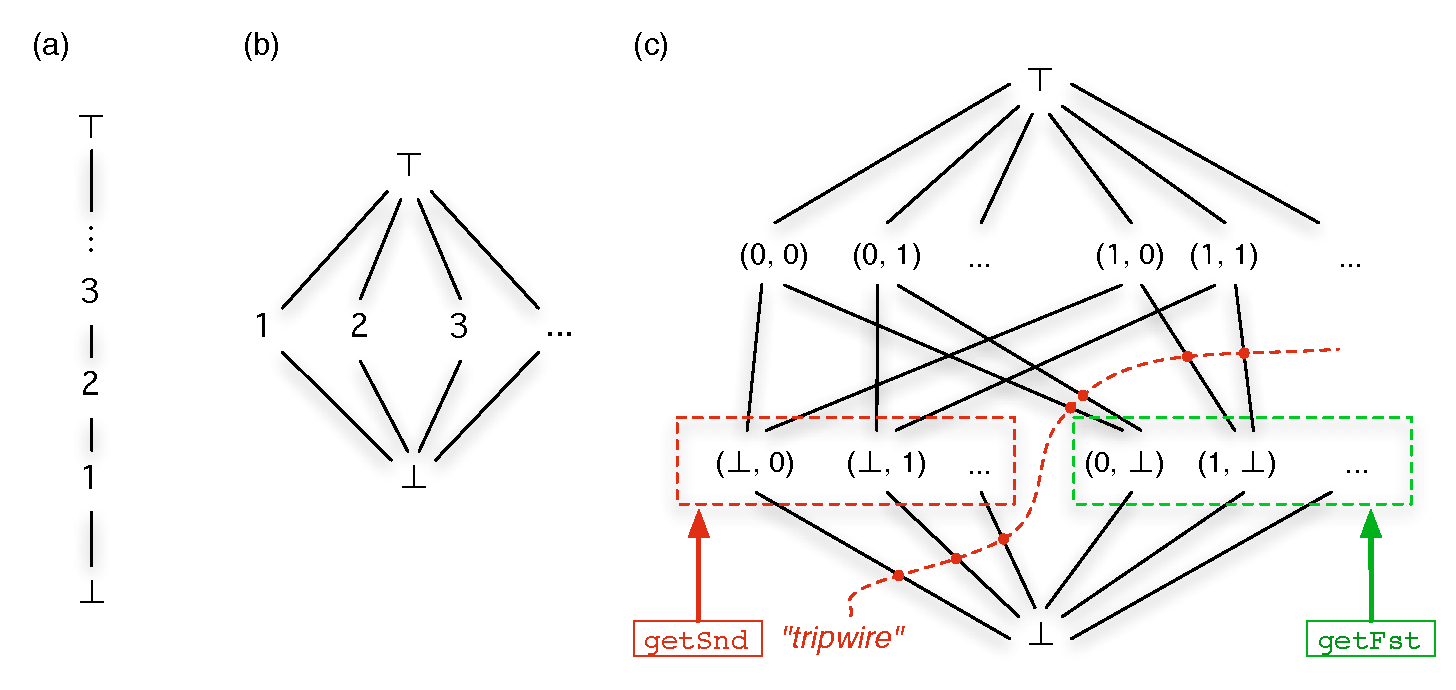
\includegraphics[width=0.75\textwidth]{figures/example-lvar-lattices.pdf} 
  \caption{Example LVar lattices: (a) positive integers ordered by
    $\leq$; (b) IVar containing a positive integer; (c) pair of
    natural-number-valued IVars, annotated with example threshold sets
    that would correspond to a blocking read of the first or second
    element of the pair.  Any state transition crossing the
    ``tripwire'' for \lstinline{getSnd} causes it to unblock and
    return a result.}

  \label{f:lattice-examples}
\end{figure}

\section{Joining forces: LVars and conflict-free replicated data types}\label{s:crdts}

In this section, I will discuss the relationship between the LVars
model I've described and the mathematical framework of
\emph{conflict-free replicated data types}, which are data structures
for reasoning about and enforcing the eventual consistency of
replicated objects in a distributed system.

\subsection{Replication and eventual consistency}

Distributed systems often involve \emph{replication} of data objects
across a number of physical locations.  Replication is of fundamental
importance in distributed systems: it makes the system more robust to
data loss and allows for good data locality.  Unfortunately, while it
would be convenient if a system of distributed, replicated objects
behaved indistinguishably from the familiar programming model in which
all data is on one machine and and all computation takes place there,
this is not and cannot be the case.  The famous CAP
theorem~\cite{gilbert-lynch-cap} of distributed computing imposes a
three-way tradeoff between:
\begin{itemize}
\item Consistency, in which every replica sees the same information;
\item Availablility, in which all information is available for both
  reading and writing by all replicas; and
\item Partition tolerance, in which the system is robust to parts of
  it being unable to communicate with one another.
\end{itemize}
An (oversimplified, but useful to a first approximation)
interpretation of the CAP theorem is the slogan, ``Consistency,
availability, and partition tolerance: pick at most two.''  In
practice, real systems must be robust to network partitions and hence
must compromise on at least one of consistency or availability.
Moreover, though, consistency, availability, and partition tolerance
are not binary properties; rather than having, for instance, either
perfect availability or no availability at all, we can choose how much
availability a system must have, then allow less conistency
accordingly.  \emph{Highly available} distributed systems (\eg,
Dynamo~\cite{dynamo}) give up on strict conistency in favor of
\emph{eventual consistency}~\cite{vogels-ec}, in which replicas may
not always agree, but if updates stop arriving, all replicas will
\emph{eventually} come to agree, given enough time.

\subsection{Resolving conflicts between replicas}

How can eventually consistent systems ensure that all replicas of an
object come to agree?  In particular, if replicas differ, how do we
determine which is ``right''?  As a straw man proposal, we could
vacuously satisfy the definition of eventual consistency by setting
all replicas to some pre-determined value---but then, of course, we
would lose all updates we had made to any of the replicas.

As a more practical proposal, we could try to determine which replica
was written most recently, and then have the last writer win.  But
this approach is also less than ideal: even if we had a way of
perfectly synchronizing clocks between replicas and could always
determine which replica was written most recently, just having the
last writer win might not make sense from a \emph{semantic} point of
view.  The developers of Dynamo, Amazon's distributed key-value store,
acknowledged this in their discussion of application-specific
mechanisms for resolving conflicts between replicas~\cite{dynamo}:
\begin{quote}
  The next design choice is who performs the process of conflict
  resolution. This can be done by the data store or the
  application. If conflict resolution is done by the data store, its
  choices are rather limited. In such cases, the data store can only
  use simple policies, such as "last write wins", to resolve
  conflicting updates. On the other hand, since the application is
  aware of the data schema it can decide on the conflict resolution
  method that is best suited for its client’s experience. For
  instance, the application that maintains customer shopping carts can
  choose to "merge" the conflicting versions and return a single
  unified shopping cart.
\end{quote}
In other words, we can take advantage of the fact that, for a
particular application, we know something about the meaning of the
data we are storing, and then parameterize the data store by a
pluggable, application-specific conflict resolution operation.

This notion of application-specific conflict resolution is not without
its problems, especially if implemented in an ad-hoc
way.\footnote{Indeed, as noted in the Dynamo article~\cite{dynamo},
  Amazon's shopping cart presents an anomaly whereby an item removed
  from a cart may re-appear!}

\lk{TODO: Write about CRDTs.}


\section{The LVish library}\label{s:lvish}

\subsection{Case studies}

\section{Related work}\label{s:related}

\subsection{Deterministic Parallel Java (DPJ)}

DPJ \cite{dpj-oopsla, dpj-hotpar09} is a deterministic language
consisting of a system of annotations for Java code.  A sophisticated
region-based type system ensures that a mutable region of the heap is,
essentially, passed linearly to an exclusive writer, thereby ensuring
that the state accessed by concurrent threads is disjoint.  DPJ does,
however, provide a way to unsafely assert that operations commute with
one another (using the @commuteswith@ form) to enable concurrent
mutation.

The LVars model differs from DPJ in that it allows overlapping shared
state between threads as the default.  Moreover, since LVar effects
are already commutative, we avoid the need for @commuteswith@
annotations.  Finally, it is worth noting that while in DPJ,
commutativity annotations have to appear in application-level code, in
LVish only the data-structure author needs to write trusted code. The
application programmer can run untrusted code that still enjoys a
(quasi-)determinism guarantee, because only (quasi-)deterministic
programs can be expressed as LVish @Par@ computations.

More recently, Bocchino \etal~\cite{dpj-popl} proposed a type and
effect system that allows for the incorporation of nondeterministic
sections of code in DPJ.  The goal here is different from ours: while
they aim to support \emph{intentionally} nondeterministic computations
such as those arising from optimization problems like branch-and-bound
search, the quasi-determinism in LVish arises as a result of schedule
nondeterminism.

\subsection{FlowPools}

Prokopec \etal~\cite{flowpools} recently proposed a data structure
with an API closely related to LVars extended with freezing and
handlers: a FlowPool is a bag that allows concurrent insertions but
forbids removals, a @seal@ operation that forbids further updates,
and combinators like @foreach@ that invoke callbacks as data
arrives in the pool.  To retain determinism, the @seal@ operation
requires explicitly passing the expected bag \emph{size} as an
argument, and the program will raise an exception if the bag goes over
the expected size.

While this interface has a flavor similar to that described in
Section~\ref{s:freezing}, it lacks the ability to detect quiescence,
which is crucial for expressing algorithms like graph traversal, and
the @seal@ operation is awkward to use when the structure of data is
not known in advance.  By contrast, the @freeze@ operation on LVars
does not require such advance knowledge, but moves the model into the
realm of quasi-determinism.  Another important difference is the fact
that LVars are \emph{data structure-generic}: both our formalism and
our library support an unlimited collection of data structures,
whereas FlowPools are specialized to bags.

\subsection{Concurrent Revisions}

The Concurrent Revisions (CR)~\cite{concurrent-revisions-haskell11}
programming model uses \emph{isolation types} \cite{isolation-types}
to distinguish regions of the heap shared by multiple mutators.
Rather than enforcing exclusive access in the style of DPJ, CR clones
a copy of the state for each mutator, using a deterministic ``merge
function'' for resolving conflicts in local copies at join points.

Variables can be annotated as being shared between a ``joiner'' thread
and a ``joinee'' thread.  Unlike the least-upper-bound writes of
LVars, CR merge functions are \emph{not} necessarily commutative;
indeed, the default CR merge function is ``joiner wins''.  Determinism
is enforced by the programming model allowing the programmer to
specify which of two writing threads should prevail, regardless of the
order in which those writes arrive.  Hence the states that such a
shared variable take on need not form a lattice.

Still, semilattices turn up in the metatheory of CR: in particular,
Burckhardt and Leijen~\cite{semantics-concurrent-revisions} show that,
for any two vertices in a CR revision diagram, there exists a
\emph{greatest common ancestor} state which can be used to determine
what changes each side has made---an interesting duality with our
model (in which any two LVar states have a lub). \lk{TODO: Write to
  them and ask them if it's a join-semilattice or a meet-semilattice!}

If versioned variables used least upper bound as their merge function
for conflicts\lk{TODO: see if ``versioned variables'' is the term they
  use}, the CR programming model would match that of LVars.  \lk{Think
  of a better way to word that last part.}  But it nevertheless
differs from the LVars model in that, in CR, effects only become
visible at the end of parallel regions. \lk{Check that this is true.}
This precludes the use of traditional lock-free data structures as a
representation for versioned variables.  LVars, on the other hand,
allow asynchronous communication within parallel regions.

\section{Road map}

I have already completed substantial work towards my thesis:

\begin{itemize}
\item \lk{Some stuff about original LVars paper}
\item \lk{Some stuff about Freeze paper}
\end{itemize}
To complete the thesis, I plan to do the following:
\begin{itemize}
\item \lk{Some stuff about CRDTs and LVars.}
\item \lk{Write the dissertation.}
\end{itemize}
\lk{Time estimates to be added.}

\bibliographystyle{plain}
\bibliography{../latex_common/refs}

\end{document}
